\chapter[Produto Desenvolvido]{Produto Desenvolvido}
% [Criar um guia de telas e explicação das funcionalidades do protótipo]

Utilizando um template para projetos C++ (github.com/CaioIcy/CPP\textunderscore Project\textunderscore Template), o Dauphine
está sendo compilado com sucesso.

\begin{figure}[h]
	\centering
	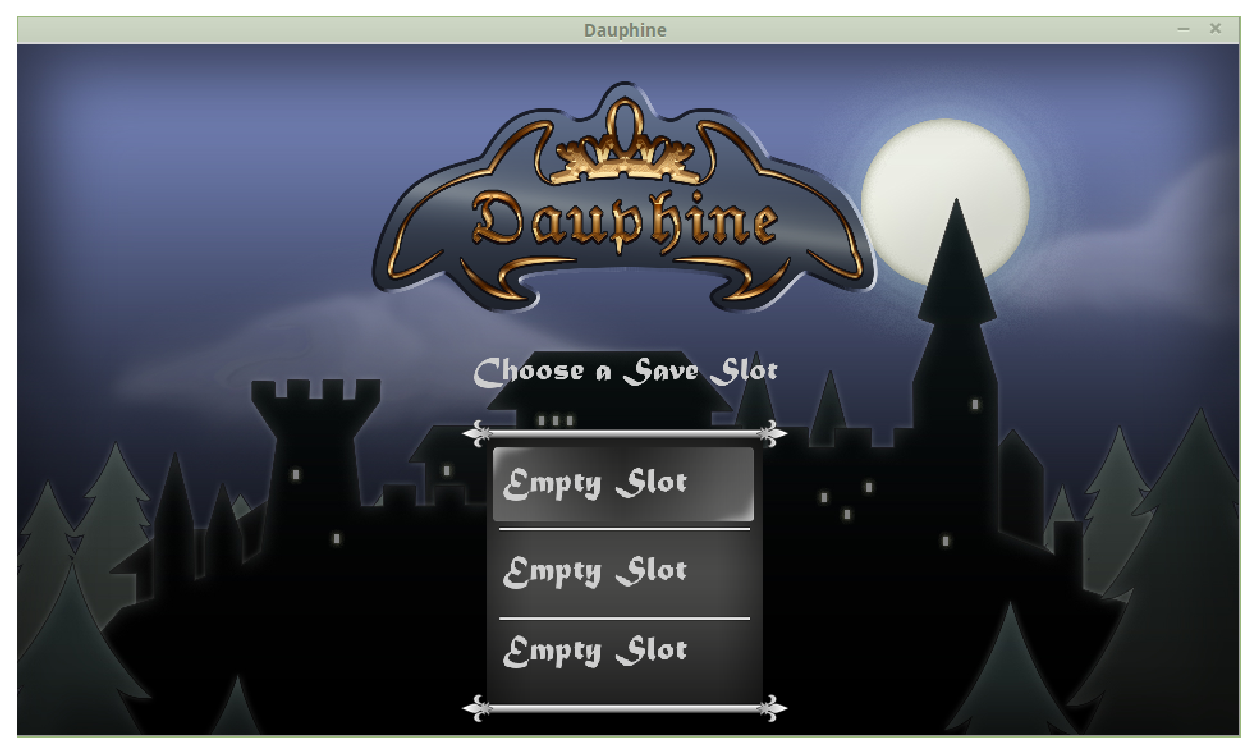
\includegraphics[width=0.8\textwidth]{figuras/vv_dauphine.eps}
	\caption{Menu de Dauphine}
	\label{img:dauphine}
\end{figure}

\begin{figure}[h]
	\centering
	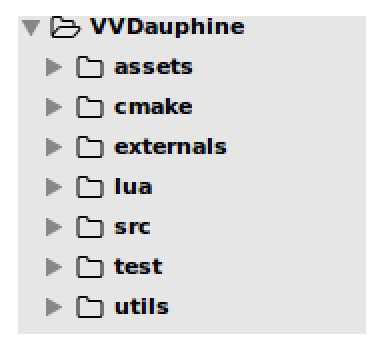
\includegraphics[width=0.4\textwidth]{figuras/vv_cp3t.eps}
	\caption{Estrutura proveniente do template de projetos C++}
	\label{img:cp3t}
\end{figure}

Já com a integração contínua configurada, os testes estão sendo executados a cada commit na branch master.

\begin{figure}[h]
	\centering
	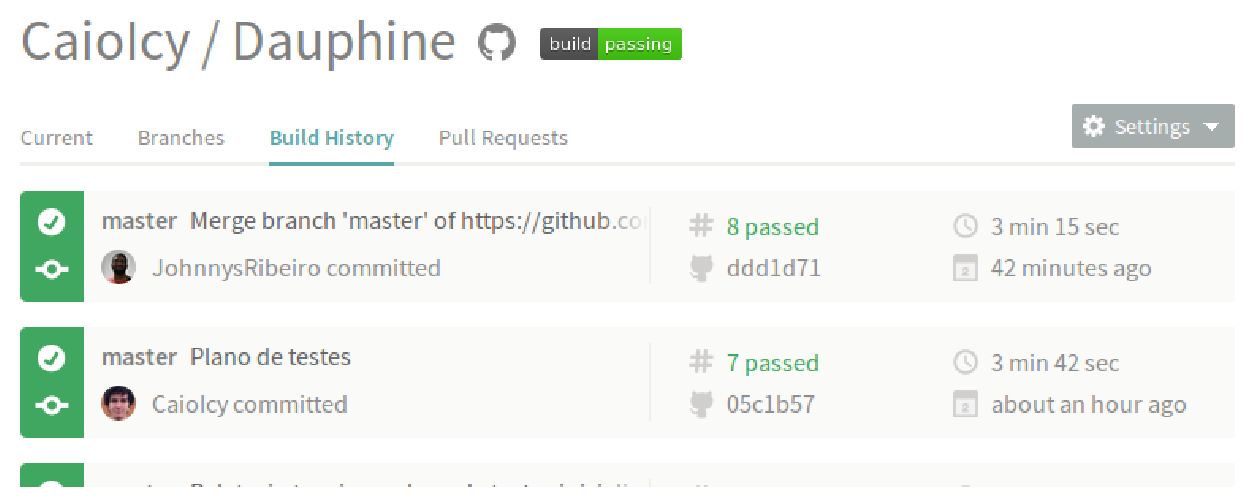
\includegraphics[width=0.8\textwidth]{figuras/vv_travis.eps}
	\caption{Histórico de builds no Travis CI}
	\label{img:travis}
\end{figure}

\begin{figure}[h]
	\centering
	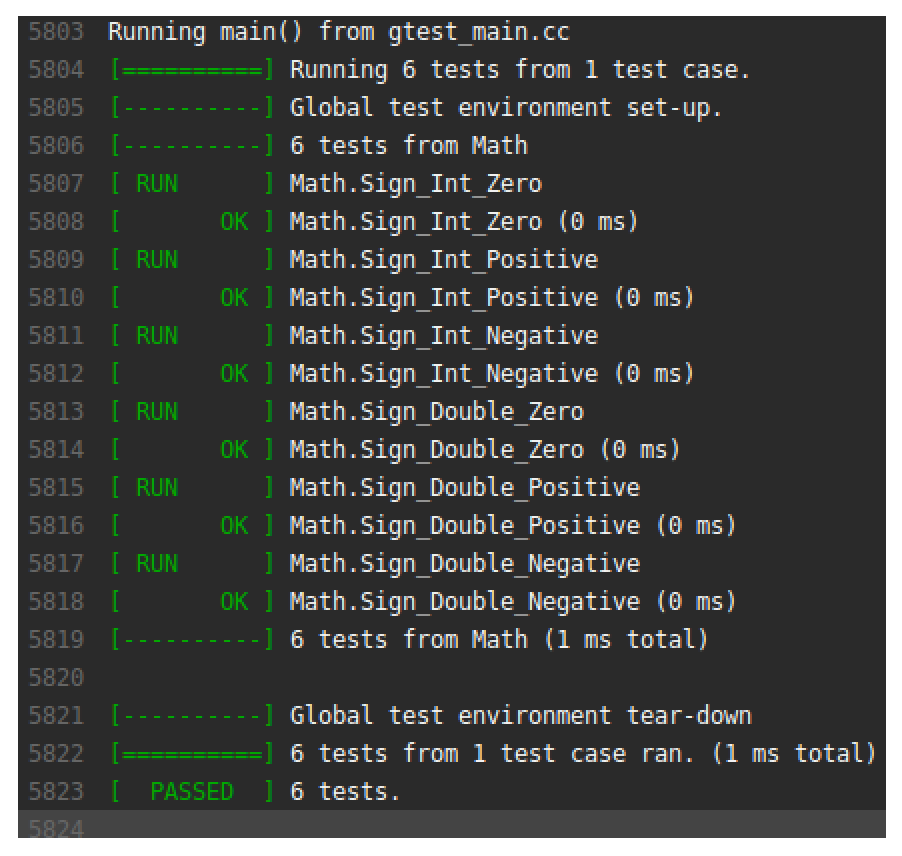
\includegraphics[width=0.6\textwidth]{figuras/vv_travis_tests.eps}
	\caption{Testes sendo executados dentro do Travis CI}
	\label{img:travis_tests}
\end{figure}

